%-----------------------------------------------------------------------------
% Name:         spoom.tex
%
% Purpose:      small paper
%
% Guide:        sigplanconf-guide.pdf
%
% Author:       Lan
%
% Created:      4 April 2014
%
%-----------------------------------------------------------------------------


\documentclass[nocopyrightspace,9pt]{sigplanconf}

% The following \documentclass options may be useful:

% preprint      Remove this option only once the paper is in final form.
% 10pt          To set in 10-point type instead of 9-point.
% 11pt          To set in 11-point type instead of 9-point.
% authoryear    To obtain author/year citation style instead of numeric.

\usepackage{amsthm}
\usepackage{amsmath}
\usepackage{balance}
\usepackage{epsfig}
\usepackage{algorithm}
\usepackage{algorithmic}
\usepackage{graphicx}
\usepackage{relsize}

\hyphenpenalty=2000   %avoid the hyphen

\newlength\myindent
\setlength\myindent{1em}
\newcommand\bindent{
  \begingroup
  \setlength{\itemindent}{\myindent}
  \addtolength{\algorithmicindent}{\myindent}
}
\newcommand\eindent{\endgroup}

\newlength\mysecindent
\setlength\mysecindent{2em}
\newcommand\quadindent{
  \begingroup
  \setlength{\itemindent}{\mysecindent}
  \addtolength{\algorithmicindent}{\mysecindent}
}
\newcommand\quadeindent{\endgroup}
\newcommand\lan[2]{{\left|{#1}\right|}_{#2}}
\newcommand\lanceil[2]{\left\lceil\frac{#1}{#2}\right\rceil}
\newcommand\bop[0]{\mathsmaller{\bigoplus}}
\newcommand\op[0]{\mathlarger{\mathop{\oplus}}}

\begin{document}

\title{Communication Cost Optimized Key Establishment Scheme Based On Secret Sharing}

\authorinfo{Lan Zongxiao}
           {National University of Defense\\Technology,Changsha,Hunan}
           {517003047qq@gmail.com}
\authorinfo{Xiageming}
           {National University of Defense\\Technology,Changsha,Hunan}
           {xiageming@126.com}

\maketitle

\begin{abstract}
With the rapid development of Wireless Sensor Networks(WSNs),
however, its security issues have become outstanding because of the
inclement deploying environment, and the open communication channel.
Due to the constraints of limited hardware resources
and computational capabilities, most of the defense mechanism are based on
symmetric key. In this paper, we present a algorithm \textit{DPC},
\textit{Data Partitioning with Coding}.Based on \textit{DPC}, we proposed a secret
sharing-based scheme to protect the
establishment of session key in WSNs. As a result, be means of optimizing the
communication cost, the scheme is suitable for WSNs.
\end{abstract}

\keywords
Secret Sharing, Wireless sensor network, Optimization

\section{Introduction}
With the increasing demand for environmental monitoring or
intelligent transmission etc. wireless sensor networks (WSNs) have been deployed
extensively. The application requirements leads to the
increase of the scale of wireless sensor network. If depend on the radio
data transmission mechanism entirely, however, the resource and energy consumption of
the sensor nodes will be too large. The effective use of end-to-end
transmission in sensor network can guarantee the efficiency and reduce the consumption.
%Due to the constraints of limited hardware resources and computational
%capabilities, most of the defense mechanism are based on symmetric key.
Due to the inclement deploying environment, and the open communication channel,
sensor network is vulnerable to attack. It's not feasible to use asymmetric
cryptography in sensor network because of the constraints of limited hardware
resources and computational capabilities\cite{carman2000constraints}.\\

Therefore adequate defense mechanism based on symmetric cryptography
should be proposed to secure the key establishment in end-to-end
transmission. Pairwise key establishment is a fundamental security service in sensor networks\cite{liu2005establishing}.
%In \cite{zhang2007random}, the authors present a random perturbation based (RPB) scheme for pairwise key %establishment in sensor networks, which is resilient to a large number of
%node compromises.
In \cite{zhu2006leap},the authors proposed schemes provided by LEAP to establish
and update keys using pairwise shared keys for each node. And the local
collaboration-based group key updating scheme has been proposed\cite{zhang2005group}.
However, in these schemes, the sensor network
ensure the security in the process of establishing and updating keys.
%In \cite{zhu2003establishing,chan2003random}, they both use threshold secret
%sharing to enhance the security.\\
In \cite{chan2003random}, the author present \textit{multipath key reinforcement}, which is based
on secret sharing to enhance the security. To reconstruct the
link key, the adversary must eavesdrop on all
the links between the key establish node and its reinforce neighbors, for all the
expanded communication cost. The analogous scheme \textit{multiple logically disjoint path} presented in
\cite{zhu2003establishing}, which is based on threshold secret sharing.\\
%However,
%we cannot simply coordinate the key update using
%the direct link between A and B since if the adversary has
%been recording all key-setup traffic, it could decrypt the keyupdate
%message after it obtained k and still obtain the new
%communication key.

Secret sharing especially threshold secret sharing requires a calculation of more
complex, such as the Lagrange interpolating polynomial\cite{Shamir:secret}.
When the key is transmitted in multiple paths, the communication cost will
expand exponentially, bring the huge energy consumption. Being aware of such
problems, in this paper, we present a communication cost optimized key
establishment scheme based on secret sharing. Optimization of communication
cost will result in security performance degradation inevitably. Our scheme makes a trade-off
between them by using a non-perfect secret sharing.
\section{Related Work}
The first secret share schemes were introduced by Shamir\cite{Shamir:secret}
and Blakley\cite{Blakley1979} in 1979. In these (k,n) threshold schemes,
the shares of any k participants are sufficient to recover the complete secret,
yet any k-1 or less shares leak nothing about the secret.
In \cite{claveirole2008securing}, the presented schemes apply secret sharing
in wireless sensor network to against aggregator compromises.
The authors design a secret multipath aggregation (SMA) scheme, to deal with security
under the contingency of compromise. Due to the constraints of limited hardware resources
and computational capabilities, however, these schemes are not suitable for sensor network.\\

In \cite{kurihara2008fast}, Kurihara presented a secure and high-speed secret sharing scheme
using XOR operation. It's an ideal secret for the recovery and the share have the
same data length. In \cite{nagai2013key}, the authors proposed a new scheme using
XOR operation, achieved high-speed processing and reduced the data size using
pseudo-random numbers. Although in these schemes, have high-speed distribution
and recover processing, their communication cost expand seriously.\\

A secret sharing scheme is non-perfect if some subsets of participants cannot recover
the secret value but have some information about it\cite{farras2014optimal}.
While in perfect secret sharing scheme, the data size of each share have a lower bound,
that is the size of the secret. Therefore, to optimize the communication cost, we
presented a \textit{non-perfect secret sharing} scheme using XOR operation.
\section{Solution Approach}
\subsection{system model}
%\textbf{Network model}.
\subsubsection*{Network model}
%\subsubsection*{system model}
In this scheme, we combine single-step key transmission protocol and secret sharing to
achieve the key establishment. And our work is based on wireless sensor network using
pre-distribution keys.\\

Single-step key transmission protocol establish key supported by
pre-distribution keys based on symmetric encryption. The processing of key establishment
between node A and B described as follows:$E_{k}(key,t_\mathsmaller{A},c)$. $E_k$
represent the symmetric encryption algorithm using
key \textit{k}, \textit{key} is the session key to be establish,
$t_\mathsmaller{A}$ represent the time stamp or Serial number, yet the c represent the authentication field.\\

%\noindent\textbf{Assumptions}.
\subsubsection*{Assumptions}
In this paper, we assume the following.

\indent1)All the sensor nodes have completed the discovery of pre-shared keys.

2)All sensor nodes are static in the processing of key establishment.

3)Each transmission path in our work is stable in the processing of key establishment.

4)Between Node A and Node B, there are n disjoint paths, and discovered
pre-shared keys no less than n.\\

%\noindent\textbf{Notations}.
\subsubsection*{Notations}
In Table \ref{tb:notation}, the notations used in this paper is described.
\begin{table}[htbp]
\caption{Notations}
\begin{tabular}{c|l}
  \hline
  Notation & Description\\ \hline
  % after \\: \hline or \cline{col1-col2} \cline{col3-col4} ...
  $\parallel$ & Concatenation of bit sequences \\
  $\oplus$ & A bit-wise XOR operation \\
  S & The secret to be share($S\in\{0,1\}^{t\cdot p},t>0$) \\
  $\theta_i$ & The i-th block divided from the origin secret \\
  $\lan{x}{n}$ & x mod n \\
  $\beta_i$ & Share given to i-th participant $P_i(i=0,\cdots,n-1)$ \\ \hline
\end{tabular}
\label{tb:notation}
\end{table}
\subsection{secret sharing-based key establishment}
To optimize the communication cost, we present a algorithm \textit{DPC}s,
\textit{Data Partitioning with Coding}.
Based on \textit{DPC algorithm}, we proposed the multipath key establishment protocol.
As shown in Figure \ref{fig:key}, that is the session key establishment between node A and node B
using \textit{DPC algorithm}. Between node A and B have established $n$ disjoint paths
$route_1,\cdots,route_n$, throuth the finding of pre-shared keys. In \textit{DPC algorithm},
we define the coding key \textit{x}, which is used to recover secret. And the share serial
number $i_k(k=1,\cdots,n)$ refer to each path $route_k$ determine the decoding order
together with the coding key. To ensure the coding key \textit{x} and the sequence of $i_k$
only relevant to node A and B, we calculate \textit{x} and sequence of $i_k$ using the
pre-shared keys between node A and B.\\

The pre-shared keys are independent between each node-pairs, feasible to calculate the coding key
and the sequence of $i_k$.
Using the pre-shared keys $k_1,k_2,\cdots,k_n$, we calculated the pseudo-random \textit{x}
and sequence of $i_k$:
\begin{equation}\label{func_f}
  \begin{split}
    &f(k_1,k_2,\cdots,k_n)=x\\
    &F(k_1,k_2,\cdots,k_n)=(i_1,i_2,\cdots,i_n)\\
  \end{split}
\end{equation}
In our scheme, $f(k_1,k_2,\cdots,k_n)$ is a multivariate hash function which has a codomain of [$0,\cdots,n-1$]. And $F(k_1,k_2,\cdots,k_n)$ is a lightweight sequence generate function:
\[F(k_1,k_2,\cdots,k_n)=(i_1,i_2,\cdots,i_n)\quad k_{i_1}\leq k_{i_2} \leq \Lambda \leq k_{i_n}\]
\begin{figure}[htbp]
\centering
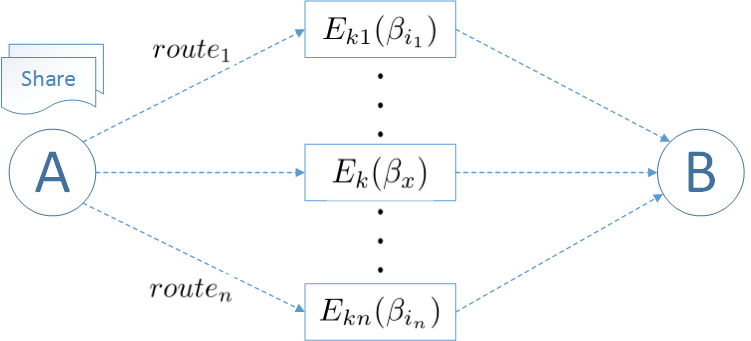
\includegraphics[width=80mm]{key.png}
\caption{Multipath key establishment based on \textit{DPC} }
\label{fig:key}
\end{figure}

Functions $f(k_1,k_2,\cdots,k_n)$ and $F(k_1,k_2,\cdots,k_n)$ were defined in all nodes, and before the
establishment of session key, node-pair use them to calculate the coding key \textit{x} and sequence of
$i_k$. The implementation of the protocol between node A
and node B contains three steps:\\

\noindent\textbf{Step 1} secret distribution:\\
Node A generate a new session key S ($S\in\{0,1\}^{n\cdot p},n>0$), and
create shares $\beta_0,\cdots,\beta_{n-1}$ from it using \textit{DPC algorithm},
in which there is one share $\beta_x$ correspond to the coding key \textit{x}.\\

\noindent\textbf{Step 2} secret transmission:\\
Encrypt each share using the pre-shared key between A and B, and each path without
using a same key. Then transfer these
encrypted shares to node B through disjoint paths $route_1,\cdots,route_n$.
Each share's transmission path is determined be the sequence of $i_k$. The i-th share
transmit through path $route_i$, for instance, the share
$\theta_{i_2}$ transmit through path $route_2$.\\

\noindent\textbf{Step 3} secret recovery:\\
Before recovery the session key, select the single key $k_x$ from the pre-distribution key pool.
When node B received shares up to n, recovery the secret using \textit{algorithm DPC},
ie. the session key between node A and Node B. From now, the multipath key establishment
protocol has achieved.\\

The multipath key establishment protocol is based on the \textit{DPC algorithm}.
This algorithm can reduced the data size of multiple secret shares significantly.
\textit{DPC} includes two parts, secret distribution and secret recovery.
The implementation detail of \textit{DPC algorithm} will be described in the following sections.
\subsection{secret distribution algorithm}
When node A and B begin to establish session key, node A generate a random value
with the same length of pre-distributed key,
which is called secret S ($S\in\{0,1\}^{n\cdot p},n>0$) in our work.
The secret distribution algorithm create secret shares from the secret S,
and then distribute them to disjoint paths.
The detail description of the distribution processing is shown as below:\\

\noindent\textbf{Step 1} Divide S into n pieces of p-bit block:\\
\begin{equation}\label{dis_1}
  S=\theta_0\parallel\theta_1\parallel\cdots\parallel\theta_{n-1}
\end{equation}
\textbf{Step 2} Make the n blocks in sequence, then execute XOR
operations within adjacent blocks, create the segment $\beta_i$:\\
\begin{equation}\label{dis_2}
  \beta_i=\theta_i \bop\theta_{\lan{i+1}{n}}(i=0,\cdots,n-1)
\end{equation}
\textbf{Step 3} Before the distribution processing, the coding key x($x\in[0,\cdots ,n-1]$)
have been calculated in node A.
Execute extra XOR operation for segment $\beta_x$, renew this segment:\\
\begin{equation}\label{dis_3}
  \beta_x=\theta_x \bop\theta_{\lan{x+1}{n}}\bop \theta_{\lan{x+\lanceil{n}{2}}{n}}
\end{equation}
From now, we have generated all share $\beta_i$ for participant $P_i(i=0,\cdots,n-1)$
\subsection{secret recovery algorithm}
After node B received all the shares, \textit{DPC algorithm} begin to recover the secret,
that is the session key. Node B calculated the coding key \textit{x} and the sequence of $i_k$
before the recovery processing, which determined the right order of decoding.
The detail description of the recovery processing is shown as below:\\

\noindent\textbf{Step 1} Execute XOR operation for the segments, recover the block $\theta_\mathsmaller{{\lan{x+\lanceil{n}{2}}{n}}}$:\\
\begin{equation}\label{rev_1}
\begin{split}
  \bop\limits_{i=0}^{n} \beta_i
  &=(\bop\limits_{i=0}^{x-1}\beta_i)\bop \beta_x
  \bop (\bop\limits_{j=x+1}^{n-1}\beta_j)\\
  &=\theta_0\bop(\bop\limits_{k=1}^{n-1}\theta_k)
  \bop\theta_0\bop\theta_{\lan{x+\lanceil{n}{2}}{n}}\\
  &=\theta_{\lan{x+\lanceil{n}{2}}{n}}
\end{split}
\end{equation}
\textbf{Step 2} Then from $y=\lan{x+\lanceil{n}{2}}{n}$, recover all the blocks in turn
until all the blocks have been recovered:\\
\begin{equation}\label{rev_2}
  \begin{split}
    &\theta_{\lan{y+1}{n}}=\theta_y\bop \beta_y\\
    &\theta_{\lan{y+2}{n}}=\theta_{\lan{y+1}{n}}\bop \beta_{\lan{y+1}{n}}\\
    &\qquad\quad\cdots\\
    &\theta_{\lan{x+1}{n}}=\theta_x\bop \beta_x \bop \theta_{\lan{x+\lanceil{n}{2}}{n}}\\
    &\qquad\quad\cdots\\
  \end{split}
\end{equation}
\textbf{Step 3} Recover secret S from all the blocks:\\
\begin{equation}\label{rev_3}
  S=\theta_0\parallel\theta_1\parallel\cdots\parallel\theta_{n-1}
\end{equation}
Then select the key $k_x$ from pre-distribution key pool, the session key $K$
between node A and B can be computed as:
\begin{equation}
  K=k_x\bop S
\end{equation}
\section{Evaluation}
In this section, we first analytically evaluate the performance of the
proposed multipath key establishment protocol based on \textit{DPC}, and
compare it to some previously proposed key establishment schemes.
Then, we analyse the security of the \textit{DPC algorithm}, estimate the
\textit{DPC algorithm} in terms of its defense capability against node compromise.
We evaluate that the proposed algorithm \textit{DPC}
can optimize the communication costs and make a trade-off of the security performance.
By means of conducting simulations, we show that the proposed algorithm \textit{DPC}
can optimize the communication cost and make a trade-off of the security performance.
\subsection{performance evaluation}
%Further, it is increasingly expensive in terms of communication
%overhead to find multiple disjoint paths that are very
%long.
%The trade-off for this benefit in the q-composite case
%is a smaller key pool size; the trade-off for the multipath
%key reinforcement scheme is increased network overhead.
We analyse the performance of the proposed multipath key establishment scheme(MKE)
in terms of computational costs and communication costs, then compare it with
the previous multipath key reinforcement scheme(MKR) and  multiple logically disjoint path scheme(MLDP).
The main results are shown in Table \ref{tb:performance}.

\subsubsection*{computational costs}
In our scheme, the main computational cost is the cost in the secret distribution and
secret recovery. Considering a secret S ($S\in\{0,1\}^{n\cdot p},n>0$), which is the session key,
$n$ is the number of disjoint paths as well as $p$ is the length of share transmit on each path.
We define L to be the length of the secret, as $L=np$.
During the distribution phase, it needs $(n+1)p$ bit-wise XOR operations. As well as during
the recovery phase, it needs $(2n-1)p+np=(3n-1)p$ bit-wise XOR operations. Node A and B both
need to calculate the
coding key x($x\in[0,\cdots ,n-1]$), which require $\lambda$ computational cost.
The overall computational costs of our scheme is $4np+2\lambda$, can also be expressed as $4L+2\lambda$.
In multipath key reinforcement scheme, it needs $nL+n\mu$ bit-wise XOR operations, in which $\mu$
is the computational cost of generating a L-bit random number.
Similar to multipath key reinforcement scheme, it needs $nL+n\mu$ bit-wise XOR operations in
multiple logically disjoint path scheme.\\

As shown in Equation \ref{func_f}, function $f(k_1,k_2,\cdots,k_n)$ is a multivariate hash function with lightweight operation. Therefore, the $\lambda$ and $\mu$ both have light effect in our comparison.
With the $n>3$, our scheme has a lower computational costs compared with the two previous schemes.

\subsubsection*{communication costs}
Each path has an average length of $h$ hops in this paper. In our scheme, node A needs to send
out $n$ shares with length of p-bit. Because of all the shares are forwarded hop-by-hop via
the path between node A and B, then the communication costs $C=n\times h \times p=hL$, which is
roughly equivalent to single path key transmission' costs.
In multipath key reinforcement scheme and multiple logically disjoint path scheme, each node need
send out $n$ L-bit shares to achieve the key establishment. Therefore, the communication costs
in these two schemes are both $C=n\times L \times h=nhL$.\\

The analysis results show that our scheme has n times of the efficiency improvement.
The trade-off for this benefit in the proposed scheme is the degradation of the security performance.
We will analyse the security performance in the next section, to show that the security degradation
is within the acceptable range.

\begin{table}[htbp]
\caption{Performance comparison to previous schemes}
\begin{tabular}{|p{9em}|p{4em}|p{4em}|p{4em}|}

  \hline
    & MKE & MKR & MLDP\\ \hline
  computational costs & $4L+2\lambda$ & $nL+n\mu$ & $nL+n\mu$\\  \hline
  communication costs & $hL$ & $nhL$ & $nhL$\\  \hline
\end{tabular}
\label{tb:performance}
\end{table}
\subsection{security evaluation}
%The secrecy of the link key k is protected by all j random
%values. Unless the adversary successfully manages to eavesdrop
%on all j paths, they will not know sufficient parts of the
%link key to reconstruct it.
To evaluate the security of the proposed multipath key establishment scheme, we
analyse the \textit{DPC algorithm} and estimate its security.
Then we use simulations to show that this scheme makes a good trade-off between
performance and security.
\subsubsection*{estimation of \textit{DPC}}
The proposed \textit{DPC algorithm} is non-perfect secret share, which inevitably leads to
security degradation. In this paper, we use coding-based secret share to control the security
degradation within acceptable range, moreover, optimize the communication costs significantly.
In our scheme, we have two objectives in security: increase the lower bound of share subset lead to
leak partial secret and increase the lower bound of share subset lead to leak complete secret.\\

Before analyse the lower bound of share subset, we define \textit{NLB} to be number leaked blocks.
In \textit{DPC algorithm}, a share subset $\Phi$ can derive partial secret only when $\beta_x \in \Phi$
and $|\Phi|\geq \lanceil{n}{2}$ (because of the space limited, not all the proofs listed).
When $|\Phi|= \lanceil{n}{2}$, the subset $\Phi$ can derive one block with probability:
\begin{equation}
  P_{(NLB=1)}=\frac{2}{C_n^{\lanceil{n}{2}}}
\end{equation}
When $\lanceil{n}{2}<|\Phi|<n$, let the subset size $|\Phi|=k$, then the probability of $r$
($1\leq r \leq {k-\lanceil{n}{2}+1}$) blocks leaked is:
\begin{equation}
  P_{(NLB=r)}=2\times \frac{C_{n-(\lanceil{n}{2}+r-1)-1}^{k-(\lanceil{n}{2}+r-1)}}{C_n^k}
\end{equation}
The share subset $\Phi$ can derive the complete secret depend on $|\Phi|=n$.
When $|\Phi|=n$, all of the shares can derive the secret apparently.

\begin{figure}[htbp]
\centering
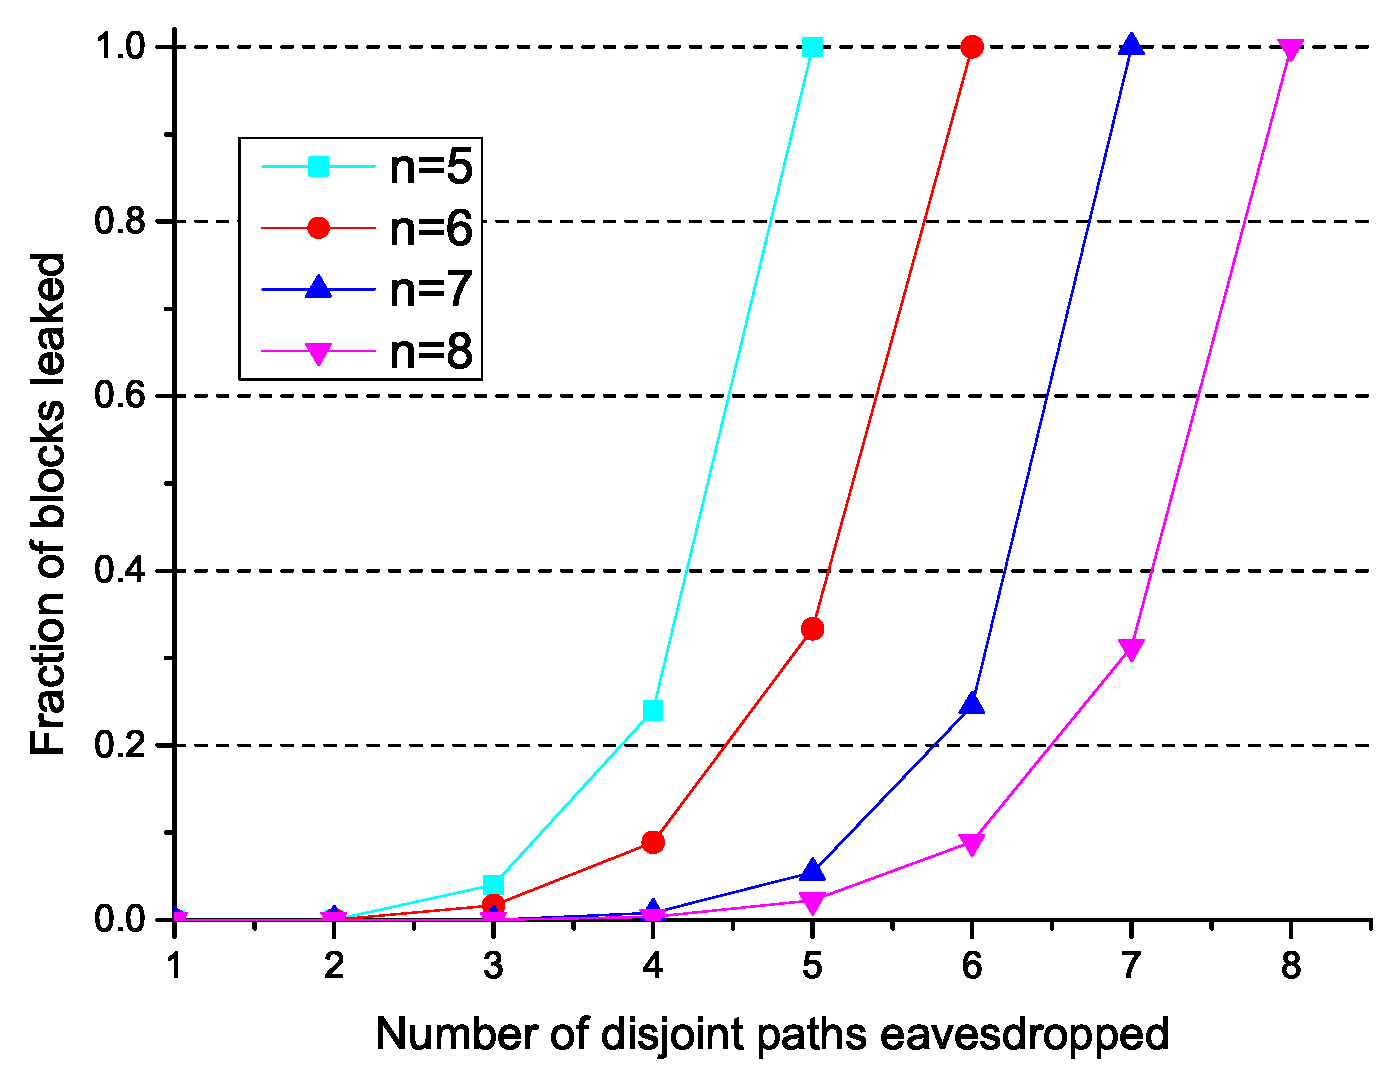
\includegraphics[width=80mm]{sdf.eps}
\caption{The fraction of blocks leaked according to subset size
of eavesdropped shares (ignore the probability of eavesdropping a disjoint path)}
\label{fig:nlb}
\end{figure}

In Figure \ref{fig:nlb}, we show that \textit{DPC algorithm} has relative security performance degradation
whereas it's based on non-perfect secret share. When the share subset $|\Phi|\leq n-1$, the adversary
has no chance to eavesdrop the link between node A and B, as well as
the adversary has no chance to eavesdrop a block if $\Phi \leq \lanceil{n}{2}$.
Even if $|\Phi| =n-1$, the fraction of
blocks leaked will not more than 0.4. By the way, as shown in Figure \ref{fig:nlb}, the scheme with
an odd number of disjoint paths has better security performance relative to which has even number
of disjoint paths.
%Taking into account the scarcity of pre-distribution keys between each node pair,
%we choose $n=5$ in this paper.

\subsubsection*{evaluation of \textit{MKE}}
We evaluate the effectiveness of the presented multipath key establishment scheme
by simulating the 10000 sensor nodes deployed on a planar field.
In our simulation, each node has 50 neighbours with the proper deployment density.
The adversary eavesdrop on each disjoint path by compromise the nodes on it.
A pairwise nodes communication is compromised only if the session key is compromised,
that is all the disjoint paths to be used to transmit the session key were compromised in
our scheme.\\

\begin{figure}[htbp]
\centering
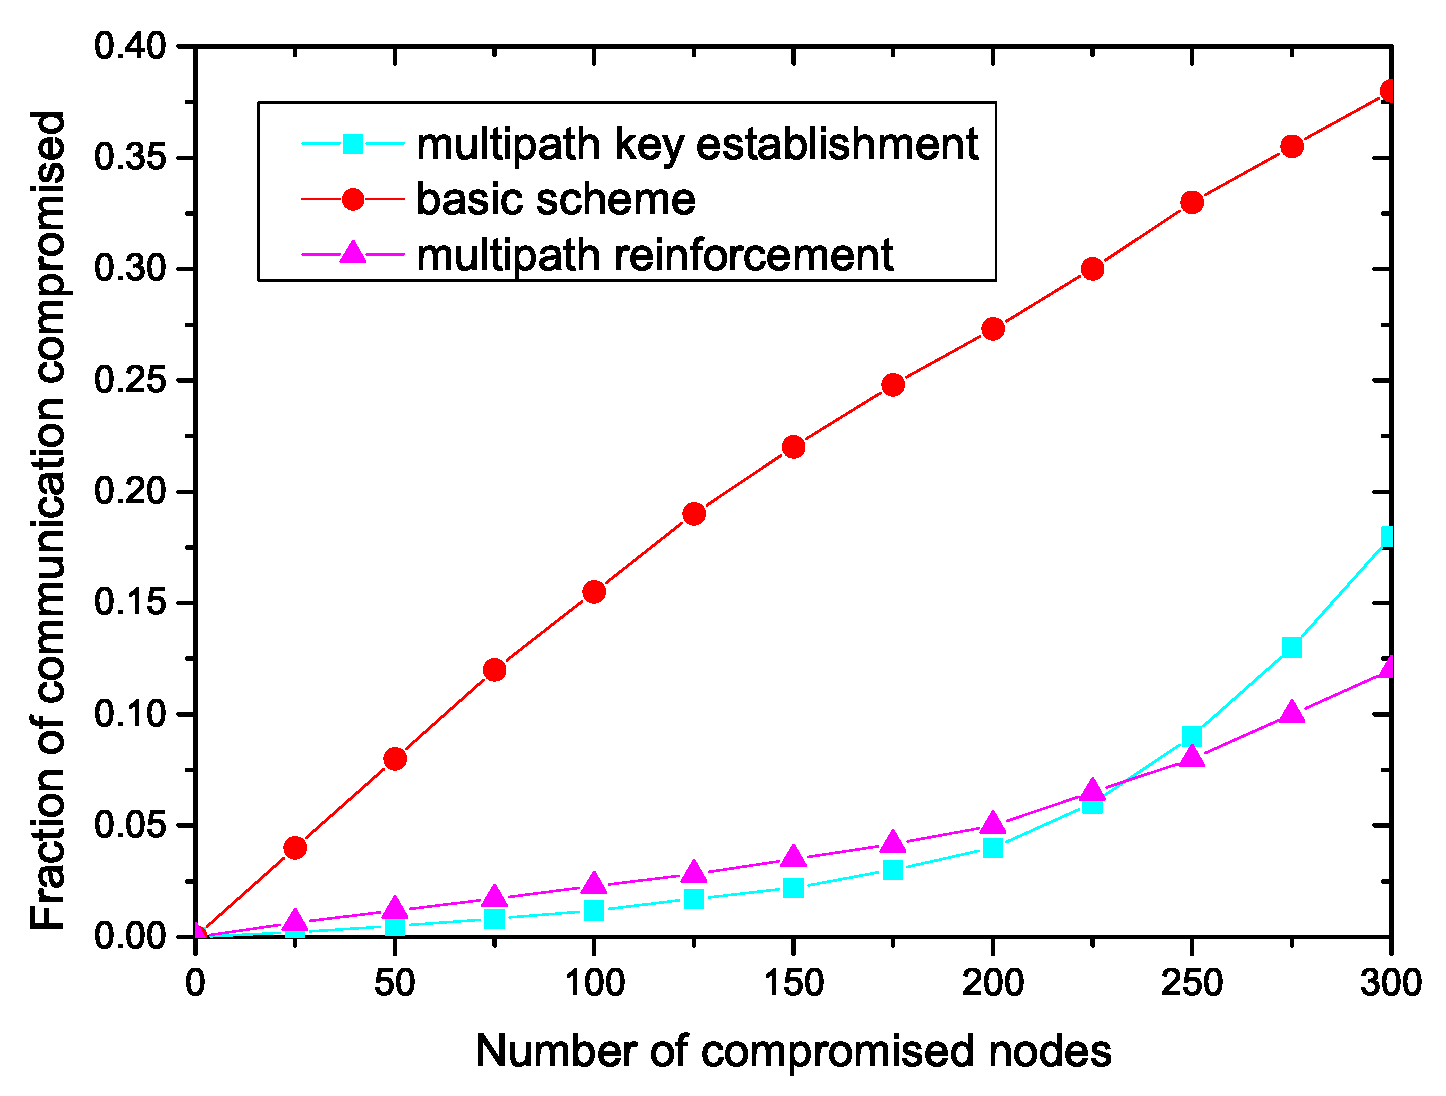
\includegraphics[width=80mm]{compromise.eps}
\caption{The fraction of blocks leaked according to subset size
of eavesdropped shares (ignore the probability of eavesdropping a disjoint path)}
\label{fig:compromise}
\end{figure}


We plot the simulation results in Figure \ref{fig:compromise}, which indicates
the fraction of communication compromised versus the number of compromised nodes.
Figure \ref{fig:compromise} shows
that our multipath key establishment scheme acts similarly to the previously proposed schemes in security.
When the number of compromised nodes less than 225, its security performance even outperform
the multipath reinforcement scheme.\\

The adversary require to eavesdrop multiple relevant keys in order to eavesdrop
the session key between node pairs. 
The trade-off for the multipath key establishment scheme is the increased communication costs.
The benefit of \textit{DPC algorithm} is remaining the security unchanged, while the communication costs
optimized significantly. In our scheme, the blocks of the secret
as well as the complete of the secret have small probability to be eavesdropped.
%Considering the probability of compromising the complete session key between node A and B,
%it acts almost similarly to the previously proposed schemes, despite potential blocks leaked.
%The multipath key establishment scheme increases the difficulty of compromising the session
%key by adversary. The adversary require to eavesdrop multiple relevant keys in order to eavesdrop
%the session key between node pairs.
%The trade-off for the multipath key establishment scheme is the increased communication costs.\\
%
%The benefit of \textit{DPC algorithm} is remaining the security unchanged, while the communication costs
%optimized significantly. In our scheme, the blocks of the secret
%as well as the complete of the secret have small probability to be eavesdropped.
\section{Conclusions}
We have presented a new multipath key establishment scheme using non-perfect secret share
for wireless sensor network. We analyse the overhead roundly to show that our scheme
optimize the communication costs and make a trade-off of the security performance.
\acks

This work is supported in part by Natural Science Foundation of China
grants 61070201.

%% We recommend abbrvnat bibliography style.
%only index by the order of ref
\bibliographystyle{IEEEtran}
\balance
\bibliography{spoom}


\end{document}

